\documentclass[11pt]{beamer}
\usetheme{CambridgeUS}
\usepackage[utf8]{inputenc}
\usepackage{amsmath}
\usepackage{amsfonts}
\usepackage{amssymb}
\usepackage[
backend=biber,
style=alphabetic,
citestyle=authoryear
]{biblatex}
\usepackage{array}
\usepackage{xcolor}

% Footnote without number
\newcommand\blfootnote[1]{%
  \begingroup
  \renewcommand\thefootnote{}\footnote{#1}%
  \addtocounter{footnote}{-1}%
  \endgroup
}
\def\boxit#1{%
  \smash{\color{red}\fboxrule=1pt\relax\fboxsep=2pt\relax%
  \llap{\rlap{\fbox{\vphantom{0}\makebox[#1]{}}}~}}\ignorespaces
}
\addbibresource{stats.bib}
\title[Bioestatística II] %optional
{ANOVA de um fator para amostras independentes}

\subtitle{CGF2046 - Bioestatística II}

\author[da Silva, Ricardo] % (optional, for multiple authors)
{R. ~R. ~da Silva\inst{1}}

\institute[FCFRP] % (optional)
{
  \inst{1}%
  Departamento de Ciências BioMoleculares\\
  Faculdade de Ciências Farmacêuticas

}

\date{\today} % (optional)

\titlegraphic{
\includegraphics[width=5.8cm]{figs/logo_final}} 

\begin{document}

%\begin{frame}
%\titlepage
%\end{frame}

%\begin{frame}
%\tableofcontents
%\end{frame}

\begin{frame}
\titlepage
\end{frame}

\begin{frame}
\label{contents}
\frametitle{Sumário}
\tableofcontents
\end{frame}

\setbeamercovered{transparent}
\begin{frame}
\frametitle{Objetivos de Aprendizado\footcite{carlson2017introduction}}
  Depois de assitir essa aula e fazer as atividades complementares, você será capaz de:
  \\~\\
  \begin{itemize}
  \uncover<1->{\item
    Identificar quando usar uma ANOVA de amostras independentes;}
  \uncover<2->{\item
    Explicar a lógica da razão F para ANOVA;}
   \uncover<3->{\item
    Explicar como o erro de medição, as diferenças individuais e os efeitos do tratamento influenciam o numerador e o denominador da razão F;}
   \uncover<4->{\item
    Escrever hipóteses nulas e de pesquisa usando símbolos e palavras;}
   \uncover<5->{\item
    Preencha uma tabela de resumo da ANOVA calculando os graus de liberdade, SQs, QMs e razão F;}
   \uncover<7->{\item
    Defina uma região crítica e determine se você deve rejeitar ou não rejeitar a hipótese nula;}
   \uncover<8->{\item
    Calcular tamanhos de efeito e descrevê-los;}
   \uncover<9->{\item
    Explicar quando e por que os testes \textit{post hoc} são necessários;}
   \uncover<10->{\item
    Resumir os resultados de uma ANOVA de amostras independentes;}                           
  \end{itemize}
\end{frame}

\setbeamercovered{transparent}
\begin{frame}
\frametitle{Objetivos de Aprendizado\footcite{carlson2017introduction}}
  Depois de assitir essa aula e fazer as atividades complementares, você será capaz de:
  \\~\\
  \begin{itemize}
   \uncover<1->{\item
    Usar \textit{software} para calcular uma ANOVA de amostras independentes, incluindo testes \textit{post hoc};}
   \uncover<2->{\item
    Interpretar a saída do \textit{software} para uma ANOVA de amostras independente.}                            
  \end{itemize}
\end{frame}

\section{ANOVA de amostras independentes}
\setbeamercovered{transparent}
\begin{frame}
\frametitle{ANOVA}
O teste t de amostras independentes e o teste t de amostras relacionadas comparam duas médias amostrais para determinar se seu desvio é maior do que seria esperado pelo erro amostral. \\~\\

Uma ANOVA é substancialmente mais flexível, pois pode \textbf{comparar duas ou mais médias} amostrais ao mesmo tempo para determinar se o desvio entre qualquer par de médias amostrais é maior do que seria esperado pelo erro amostral.

\end{frame}

\setbeamercovered{transparent}
\begin{frame}
\frametitle{Lógica da ANOVA}
Todos os testes de significância que você aprendeu até agora  compartilham uma lógica comum. \\~\\ 

A ANOVA analisa a variância das observação entre e dentro das condições da VI, numa tentativa de determinar se as diferentes condições de tratamento afetam os valores de forma diferente. Para compreender essa lógica, devemos entender as três fontes que afetam a variância das observações:
\end{frame}

\setbeamercovered{transparent}
\begin{frame}
\frametitle{Lógica da ANOVA}
A ANOVA analisa a variância das observação entre e dentro das condições da VI, numa tentativa de determinar se as diferentes condições de tratamento afetam os valores de forma diferente. Para compreender essa lógica, devemos entender as três fontes que afetam a variância das observações:

\begin{enumerate}
\item \textbf{Erro de medição}: Sempre haverá variação nas observações entre as unidades amostrais porque as variáveis não podem ser medidas perfeitamente.
\item \textbf{Diferenças individuais}: Sempre haverá variação nas observações entre as unidades amostrais porque as unidades são naturalmente diferentes entre si.
\item \textbf{Efeito do tratamento}: Pode haver variação nas observações entre os grupos porque estes experimentaram diferentes condições (VI) ou tratamentos.
\end{enumerate}
\end{frame}

\setbeamercovered{transparent}
\begin{frame}
\frametitle{Lógica da ANOVA}
As duas primeiras fontes de variância nas observações, erro de medição e diferenças individuais, estarão sempre presentes. Essas duas fontes de variação são frequentemente chamadas coletivamente de variação de erro porque ambos são componentes do erro amostral.\\~\\

Os pesquisadores usam a ANOVA para estimar a quantidade de variação das observações criada pelas diferentes condições de tratamento (VI).
\end{frame}

\setbeamercovered{transparent}
\begin{frame}
\frametitle{Lógica da ANOVA}
Duas representações da fórmula conceitual para uma ANOVA independente são mostradas a seguir:
 
\[F = \frac{Variabilidade\quad entre\quad condicoes\quad de\quad tratamento}{Variabilidade\quad dentro\quad das\quad condicoes\quad de\quad tratamento}\]
 
\[F = \frac{Efeito\quad do\quad tratamento\quad \&\quad diferencas\quad individuais\quad \&\quad erro\quad de\quad medicao}{Diferencas\quad individuais\quad \&\quad Erro\quad de\quad medicao}\]

O numerador da razão F é a variabilidade nas observações que existe entre os diferentes grupos de tratamento (ou seja, condições da VI), que é chamada de variabilidade entre grupos ou variabilidade entre tratamentos.
\end{frame}

\setbeamercovered{transparent}
\begin{frame}
\frametitle{Lógica da ANOVA}
Por exemplo, se uma condição tivesse valores observados altos e outra condição tivesse valores observados baixos, haveria muita variabilidade entre grupos. No entanto, se todas as condições tivessem valores semelhantes, haveria pouca variabilidade entre grupos. \\~\\
No entanto, alguma da variabilidade entre grupos é sempre causada por diferenças individuais e erros de medição. Assim, o denominador da razão F, consiste em efeitos de diferenças individuais e erro de medição.
\end{frame}

\setbeamercovered{transparent}
\begin{frame}
\frametitle{Lógica da ANOVA}
Imagine uma situação em qual o efeito do tratamento cria variância zero (ou seja, o tratamento não funciona). 

\[F = \frac{0\quad \&\quad diferencas\quad individuais\quad \&\quad erro}{Diferencas\quad individuais\quad \&\quad erro}\]

Portanto, 
\begin{itemize}
\item Se o tratamento não criar variabilidade nas observações, espera-se que a ANOVA produza um valor estatístico F próximo de 1;
\item Por outro lado, se os diferentes tratamentos criarem muita variabilidade nas pontuações, espera-se que o valor F seja substancialmente maior que 1;
\item Um valor ANOVA F não pode ser negativo porque é a razão de duas variâncias, e as variâncias devem ser positivas. 
\end{itemize}
  
\end{frame}

\setbeamercovered{transparent}
\begin{frame}
\frametitle{Um exemplo de problema para ANOVA}

\textbf{Exemplo:} Suponha que você queira comparar a terapia cognitivo-comportamental (TCC) e a terapia psicodinâmica (TPD) como tratamentos para a depressão, um terceiro grupo funciona como grupo controle e não recebe tratamento (NT). Você identifica uma amostra de pessoas com depressão grave e as divide aleatoriamente em três grupos diferentes. Os valores de depressão encontrados para cada grupo estão listados na Tabela 11.1. 

\begin{center}
\begin{tabular}{ ccc } 
 \hline
TCC & TPD & NT\\
\hline
 5 & 16 & 14\\
 9 & 17 & 19\\
 11 & 18 & 16\\
 6 & 13 & 9\\
 2 & 10 & 15\\
 15 & 19 & 25\\
 $\bar{x}_1 = 8.00$ & $\bar{x}_2 = 15.50$ & $\bar{x}_3 = 16.333$\\
 $DP_1 = 4.65$ & $DP_2 = 3.39$ & $DP_3 = 5.35$\\
 \hline
\end{tabular}
\end{center}
\end{frame}

\setbeamercovered{transparent}
\begin{frame}
\frametitle{Etapa 1: examinar as pressuposições estatísticas}

Todos os testes de hipóteses são baseados em suposições específicas e, se essas suposições forem violadas, esses testes podem produzir resultados enganosos.\\~\\
Os quatro pressupostos básicos são:

\begin{enumerate}
\item independência dos dados;
\item medição apropriada das variáveis para análise;
\item normalidade das distribuições;
\item homogeneidade da variância.
\end{enumerate}

\end{frame}

\setbeamercovered{transparent}
\begin{frame}
\frametitle{Etapa 1: examinar as pressuposições estatísticas}

Os quatro pressupostos básicos são:

\begin{enumerate}
\item \textbf{independência dos dados:} os valores de depressão dos indivíduos devem ser medidos sem que a medição de um participante influencie o de outro;
\item \textbf{medição apropriada:} variável independente (VI) \(\Rightarrow\) identifica como os três tratamentos terapêuticos são diferentes, variável dependente (VD) \(\Rightarrow\) pontuação de depressão, é medida como uma variável quantitativa;
\item \textbf{normalidade das distribuições:}  para fins didáticos as distribuições tendem a ter formato normal e, portanto, essa suposição provavelmente é atendida;
\item \textbf{homogeneidade da variância:} utilizamos a regra geral de se nenhuma de suas condições tenha um desvio padrão o dobro de outra.
\end{enumerate}

\end{frame}

\setbeamercovered{transparent}
\begin{frame}
\frametitle{Etapa 2: expor as hipóteses nulas e de pesquisa simbolicamente e verbalmente}

O teste t de amostras independentes determina se a diferença das média é significativamente diferente de 0.

\begin{center}
\begin{tabular}{ m{2cm}|m{3cm}|m{2cm}|m{3cm} } 
 \hline
 Tipo de Hipótese & Simbólico & Vebal & Diferença entre médias amostral e populacional\\
  \hline
 Hipótese nula & $H_0:\mu_1=\mu_2=...=\mu_K;$ & Médias $\approx$ para todas populações & Erro amostral \\
 Hipótese de pesquisa & $H_a:\mu_i \neq \mu_j.$ & Médias $\neq$ para pelo menos um par & Um ou mais tratamentos têm efeito  \\ 
 \hline
 \hline
\end{tabular}
\end{center}

\end{frame}

\begin{frame}
\frametitle{Etapa 3: Definir o valor crítico de F}
Especificamente, você precisará dos graus de liberdade entre tratamentos (\(gl_{entre}\)) e dos graus de liberdade dentro dos tratamentos (\(gl_{dentro(error)}\)) para encontrar o valor F crítico:

\(gl_{entre} = g - 1\), entre onde g representa o número de grupos/condições de tratamento, e

\(gl_{dentro} = N-g\), onde N representa o número de valores em estudo inteiro.

Neste caso, o \(gl_{entre} = 3 - 1 = 2\), e o \(gl_{dentro} = 18 - 3 = 15\).\\~\\

\begin{columns}
\begin{column}{0.5\textwidth}
   Excerto da tabela F
\begin{center}
\begin{tabular}{cccc} 
 \hline
gl & 1 & 2 & 3\\
14 & 4.600100 &	4.543100 & 4.494000\\
\boxit{2.5in} 15 &	3.738900 & 3.682300 & 3.633700\\
16 & 3.343900 & 3.287400 & 3.238900\\
 \hline
\end{tabular}
\end{center}   
   
   
\end{column}
\begin{column}{0.5\textwidth}  %%<--- here
   \begin{itemize}
   \item Se o valor F for igual ou maior que o valor F crítico, você rejeita a hipótese nula.
   \end{itemize}
\end{column}
\end{columns}
\end{frame}

\setbeamercovered{transparent}
\begin{frame}
\frametitle{Etapa 4: calcular a estatística do teste (teste t de amostras independentes)}
\textit{4a. Calcule o desvio entre as duas médias amostrais}\\~\\

Existem dois termos no numerador da estatística t. A primeira $(\bar{x}_1 - \bar{x}_2)$ é a diferença entre as duas médias amostrais. O segundo $(\mu_1 - \mu_2)$ é a diferença entre as duas populações, assumindo que a hipótese nula é verdadeira. Assim, o numerador é simplesmente a diferença observada entre as duas médias amostrais:

\[(\bar{x}_1 - \bar{x}_2) = ( 20.17 - 18.67) = 1.50\]

\end{frame}

\setbeamercovered{transparent}
\begin{frame}
\frametitle{Etapa 4: calcular a estatística do teste (teste t de amostras independentes)}
4b. Calcule o erro de amostragem esperado
\[SQ_1 = \frac{1}{N-1}\sum_{i=1}^n(x_{1i} - \bar{x}_1)^2 = 1.767\]
\[DP_1 = \sqrt{1.767} = 1.329\]
\[SQ_2 = \frac{1}{N-1}\sum_{i=1}^n(x_{1i} - \bar{x}_1)^2 = 2.267\]
\[DP_2 = \sqrt{2.267} = 1.506\]

\end{frame}

\setbeamercovered{transparent}
\begin{frame}
\frametitle{Etapa 4: calcular a estatística do teste (teste t de amostras independentes)}
4b. Calcule o erro de amostragem esperado\\~\\
Quando apropriado, agrupar as variações tornará seu teste de significância mais preciso. A fórmula para a variância agrupada é a seguinte:

\[SQ_p = \frac{(n_1-1)SQ_1+(n_2-1)SQ_2}{(n_1-1)+(n_2-1)} = \frac{(6-1)1.767+(6-1)2.267}{(6-1)+(6-1)}=2.02\]
O método de cálculo do erro amostral que assume a homogeneidade da variância utiliza a variância agrupada para determinar o erro padrão estimado da diferença média ($SEM_i$)

\[SEM_i = \sqrt{\frac{SD_p}{n_1}+\frac{SD_p}{n_2}} = \sqrt{\frac{2.02}{6}+\frac{2.02}{6}} = 0.82\]

\end{frame}

\setbeamercovered{transparent}
\begin{frame}
\frametitle{Etapa 4: calcular a estatística do teste (teste t de amostras independentes)}

\textit{4c. Calcule a estatística do teste (teste t independente)}\\~\\

O teste t de amostras independente é a razão entre o desvio observado entre as duas médias amostrais dividido pelo erro padrão estimado da diferença média:

\[t = \frac{\bar{x}_1-\bar{x}_2}{SEM_i} =  \frac{20.17 - 18.67}{0.82} = 1.83\]

O valor t obtido não é suficientemente grande para rejeitar a hipótese nula e, portanto, você não rejeita a hipótese nula.
%\begin{center}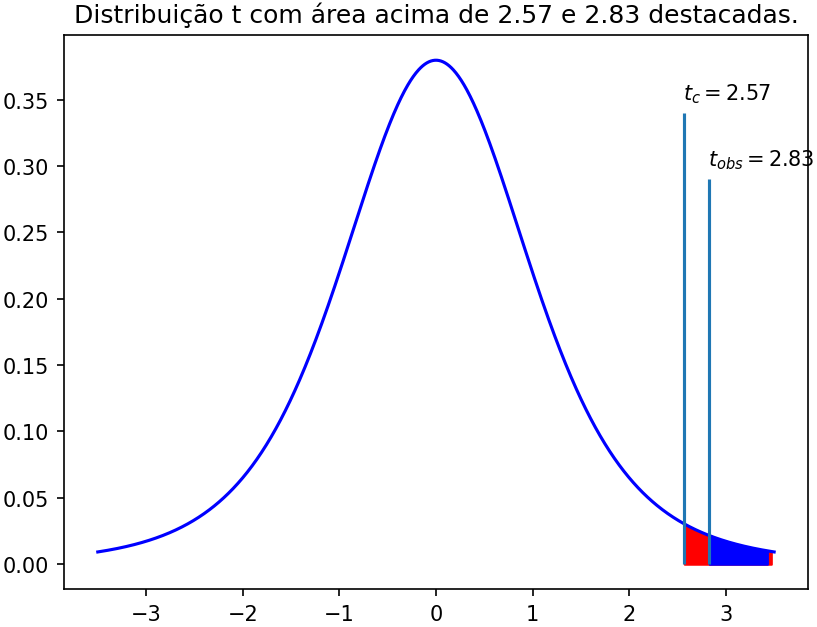
\includegraphics[width=0.55\linewidth]{figs/regiao_critica_observada_t_rel} \end{center}

\end{frame}


\setbeamercovered{transparent}
\begin{frame}
\frametitle{Etapa 5: calcule o tamanho do efeito e descreva se o seu grau}
A fórmula para calcular o tamanho do efeito de um teste t independente é semelhante à de um teste t de amostra única. No entanto, ao calcular d, o denominador é a variância combinada. 
\begin{align*}
d = \frac{\bar{x}_1 - \bar{x}_2}{\sqrt{SQ_p}} = \frac{20.17-18.67}{\sqrt{2.02}} = 1.06
\end{align*}
Quando a hipótese nula não é rejeitada e ainda assim houve um tamanho de efeito médio ou grande, o tamanho da amostra utilizado no estudo pode ter sido pequeno para que o teste estatístico ou o tamanho do efeito sejam confiáveis. Ao interpretar os resultados de qualquer estudo, também é importante considerar os resultados de outros estudos semelhantes.

\end{frame}

\setbeamercovered{transparent}
\begin{frame}
\frametitle{Etapa 5: calcule o tamanho do efeito e descreva se o seu grau}
A melhor maneira de interpretar qualquer tamanho de efeito é compará-lo com os tamanhos de efeito produzidos por estudos semelhantes na literatura de pesquisa. Se você não conseguir encontrar estudos semelhantes na literatura para fornecer uma referência, poderá usar as diretrizes gerais sugeridas por Cohen (1992) para interpretar os tamanhos dos efeitos na Tabela 6.2.

\begin{center}
\begin{tabular}{cc} 
 \hline
d  & Tamanho estimado do efeito\\
 \hline
Perto de 0.2 & Pequeno \\
Perto de 0.5 & Médio \\
Perto de 0.8 & Grande \\
 \hline
\end{tabular}
\end{center}   

\end{frame}

\setbeamercovered{transparent}
\begin{frame}
\frametitle{Etapa 6: Interpretando os Resultados do Teste de Hipóteses}

O parágrafo a seguir resume os resultados desses testes:\\~\\
Não houve diferença significativa entre as pontuações de memória daqueles que obtiveram as descrições verbais $(\bar{x}_1 = 20.17, DP_1 = 1.33)$ e daqueles que não obtiveram $(\bar{x}_2 = 18.67, DP_2 = 1.51)$, $t_{(10)} = 1.83$, $p > 0.05$, d = 1.06. No entanto, é importante notar que os tamanhos amostrais eram pequenos, portanto este estudo deve ser repetido com tamanhos amostrais maiores antes de serem tiradas conclusões.
\end{frame}

\begin{frame}
\frametitle{Exemplo de teste t de amostras independentes (unicaudal)}
\textbf{Exemplo:} Os "aprendizes visuais" têm melhor memória para informações visuais do que os "aprendizes verbais"?
\begin{itemize}
\item Vinte e nove "aprendizes verbais" e 31 "aprendizes visuais" voluntariaram-se para participar num estudo que investigou esta questão; 
\item Todos os alunos foram apresentados a desenhos de linhas simples e, em seguida, foram solicitados a recriar tantos desenhos de linhas quanto conseguissem lembrar;
\item Você usa corretamente um teste t independente unilateral com um nível \(\alpha=0.05\) para determinar se "aprendizes visuais" se lembram mais dos desenhos de linha do que "aprendizes verbais".
\end{itemize}
Grupo 1: Grupo de Aprendizes Verbais:\(\bar{x}_1 = 15.00; DP_1 = 1.41, n_1 = 29\)
\\~\\
Grupo 2: Grupo de Aprendiz Visual:\(\bar{x}_2 = 15.25; DP_2 = 1.67, n_2 = 31\)

\end{frame}

\setbeamercovered{transparent}
\begin{frame}
\frametitle{Teste t de Amostras Independentes}

\begin{center}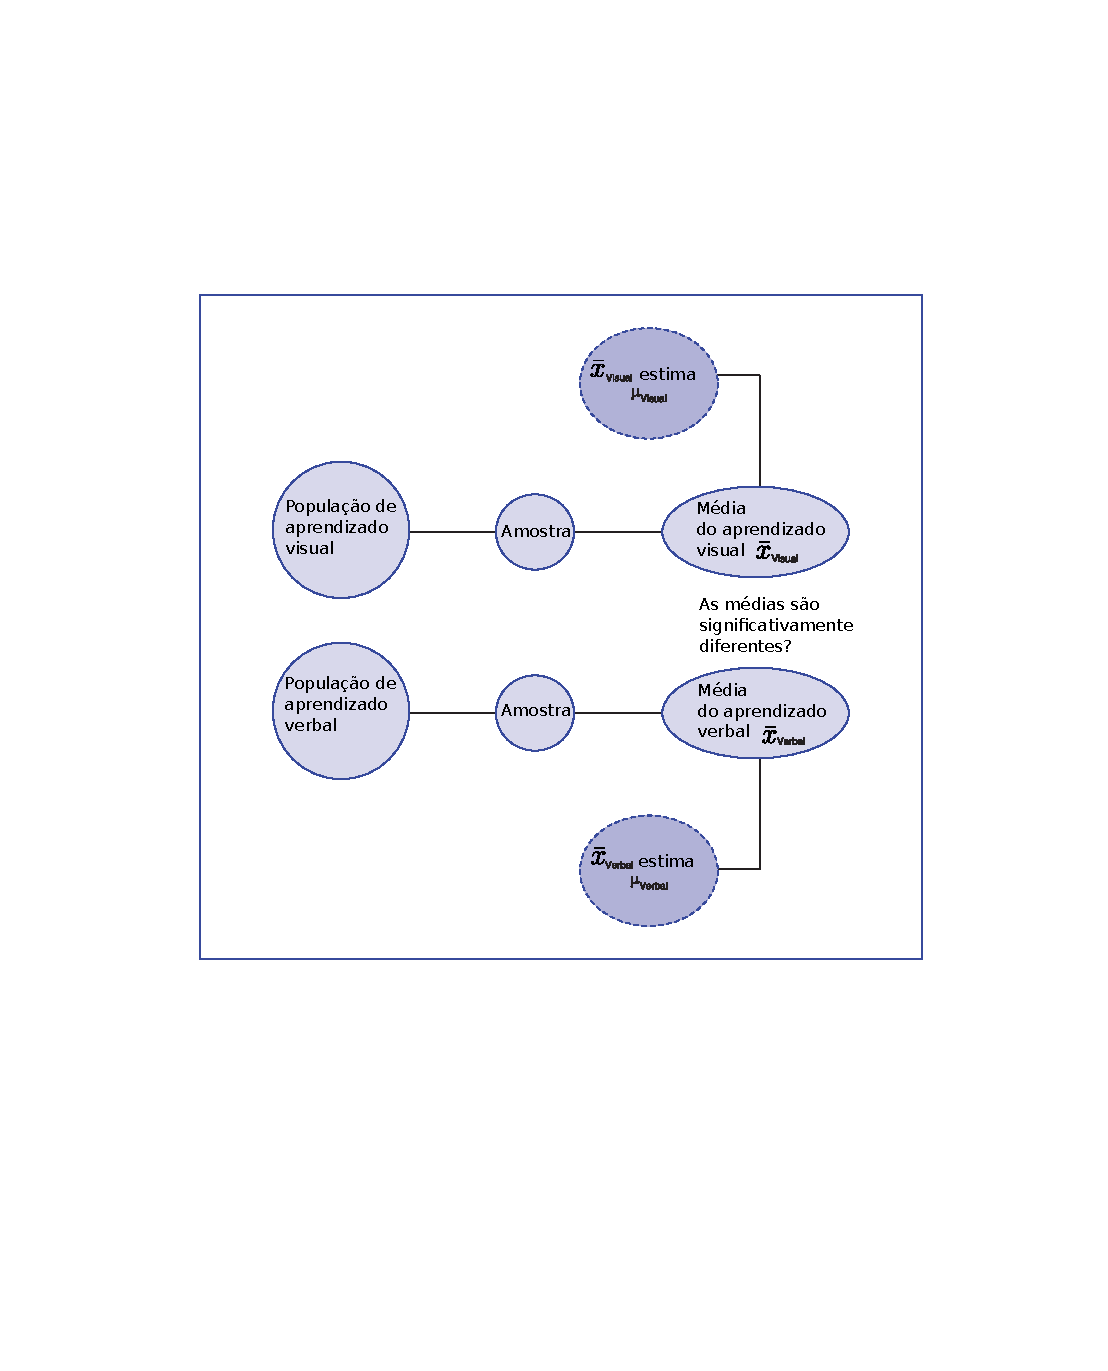
\includegraphics[width=0.7\linewidth]{figs/fig10.3} \end{center}

\end{frame}



\setbeamercovered{transparent}
\begin{frame}
\frametitle{Etapa 1: examinar as pressuposições estatísticas}

Todos os testes de hipóteses são baseados em suposições específicas e, se essas suposições forem violadas, esses testes podem produzir resultados enganosos.\\~\\
Os quatro pressupostos básicos são:

\begin{enumerate}
\item independência dos dados;
\item medição apropriada das variáveis para análise;
\item normalidade das distribuições;
\item homogeneidade da variância.
\end{enumerate}

\end{frame}

\setbeamercovered{transparent}
\begin{frame}
\frametitle{Etapa 1: examinar as pressuposições estatísticas}

Os quatro pressupostos básicos são:

\begin{enumerate}
\item \textbf{independência dos dados:} A VI, aprendizes verbais ou visuais, identifica dois grupos/condições diferentes;
\item \textbf{medição apropriada:} variável independente (VI) \(\Rightarrow\) aprendizes verbais ou visuais, variável dependente (VD) \(\Rightarrow\) número de desenhos de lembrados corretamente, é medido em como uma variável quantitativa;
\item \textbf{normalidade das distribuições:} as distribuições das pontuações de memória tendem a ter formato normal e, portanto, essa suposição provavelmente é atendida;
\item \textbf{homogeneidade da variância:} utilizamos a regra geral de que se o desvio padrão numa condição for o dobro do de outra condição, esta suposição pode ser violada.
\end{enumerate}

\end{frame}

\setbeamercovered{transparent}
\begin{frame}
\frametitle{Etapa 2: expor as hipóteses nulas e de pesquisa simbolicamente e verbalmente}

O teste t de amostras independentes determina se a diferença das média é significativamente diferente de 0.

\begin{center}
\begin{tabular}{ m{2cm}|m{3cm}|m{2cm}|m{3cm} } 
 \hline
 Tipo de Hipótese & Simbólico & Vebal & Diferença entre médias amostral e populacional\\
  \hline
 Hipótese nula & $H_0:\mu_1=\mu_2;$ ou & Diferença da médias $\approx$ 0 & Erro amostral \\
 & $H_0:\mu_1-\mu_2=0;$ & &\\
 Hipótese de pesquisa & $H_a:\mu_1 < \mu_2$ ou & Diferenças médias $<$ 0 & Aprendizes visuais lembram mais  \\ 
  & $H_a:\mu_1-\mu_2 < 0;$ & &\\
 \hline
 \hline
\end{tabular}
\end{center}

\end{frame}

\begin{frame}
\frametitle{Etapa 3: Use o tamanho da amostra para calcular os graus de liberdade e defina as regiões críticas}
Depois de saber o tamanho da amostra de um estudo, você precisa calcular seus graus de liberdade (gl). A fórmula do gl para teste t de amostras independente é $gl = (n_1 - 1) + (n_2 - 1)$, onde $n_1$ e $n_2$ representam os tamanhos amostrais das duas amostras, espectivamente. Portanto, neste caso,
\[gl = (n_1-1)+(n_2-1) = (29 - 1)+(31 - 1) = 58\]

\begin{columns}
\begin{column}{0.5\textwidth}
   Excerto da tabela t unilateral\\~\\

\begin{center}
\begin{tabular}{ccc} 
 \hline
gl & $\alpha = .05$ & $\alpha = .01$\\
57 & 1.672000 &	2.393600\\
\boxit{1.7in} 58 & 1.671600 & 2.392400\\
59 & 1.671100 &	2.391200\\
 \hline
\end{tabular}
\end{center}   
   
   
\end{column}
\begin{column}{0.5\textwidth}  %%<--- here
   \begin{itemize}
   \item O valor de corte de \(\alpha= .05\) define a região crítica, os valores t são improváveis se o valor nulo for verdadeiro.
   \end{itemize}
\end{column}
\end{columns}
\end{frame}

\setbeamercovered{transparent}
\begin{frame}
\frametitle{Etapa 4: calcular a estatística do teste (teste t de amostras independentes)}
\textit{4a. Calcule o desvio entre as duas médias amostrais}\\~\\

\[(\bar{x}_1 - \bar{x}_2) = (15.00-15) = -0.25\].

\textit{4b. Calcule o erro médio de amostra esperado}

\[SQ_p = \frac{((n_1-1)SQ_1+(n_2-1)SQ_2)}{(n_1-1)+(n_2-1)} = 2.402\]

\[SEM_i = \sqrt{\frac{SQ_p}{n_1}+\frac{SQ_p}{n_2}} = 0.4\]
\end{frame}

\setbeamercovered{transparent}
\begin{frame}
\frametitle{Etapa 4: calcular a estatística do teste (teste t de amostras independentes)}
\textit{4c. Calcule a estatística do teste (teste t de amostras independentes)}\\~\\

Novamente, o cálculo do teste t é idêntico a um teste bicaudal:

\[t = \frac{(\bar{x}_1 - \bar{x}_2)}{SEM_i} = \frac{(15 - 15.25)}{0.40} = -0.63\]

O valor t obtido de -0.63 não está mais longe de zero do que o valor crítico de -1.6716. Portanto, você não rejeita a hipótese nula.
\end{frame}

\setbeamercovered{transparent}
\begin{frame}
\frametitle{Etapa 5: calcule o tamanho do efeito e descreva se o seu grau}
Novamente, calcular o tamanho do efeito para testes unicaudais e bicaudais é idêntico:
 
\begin{align*}
d = \frac{\bar{x}_1 - \bar{x}_2}{\sqrt{SQ_p}} = \frac{15.00-15.25}{\sqrt{2.402}} = -0.16
\end{align*}

\end{frame}


\setbeamercovered{transparent}
\begin{frame}
\frametitle{Etapa 6: Interpretando os Resultados do Teste de Hipóteses}

As frases a seguir resumem os resultados deste estudo:\\~\\

Ao contrário da previsão da teoria dos estilos de aprendizagem, os alunos visuais $(\bar{x} = 15.25, DP = 1.41)$ não aprenderam significativamente mais informações visuais do que os alunos verbais $(\bar{x} = 15.00, DP = 1.67)$, $t_{(58)} = -0.63$, $p > 0.05$ (unicaudal), d = -0.16. O resultado nulo do estudo é consistente com os resultados nulos encontrados por vários outros pesquisadores que investigam estilos de aprendizagem. Coletivamente, os resultados nulos de vários estudos sobre estilos de aprendizagem sugerem fortemente que há muito pouco, ou nenhum, mérito na teoria da aprendizagem dos estilos de aprendizagem.

\end{frame}

\setbeamercovered{transparent}
\begin{frame}
\frametitle{Comparação de Duas Médias\footcite{magalhaes2002noccoes}}

\begin{center}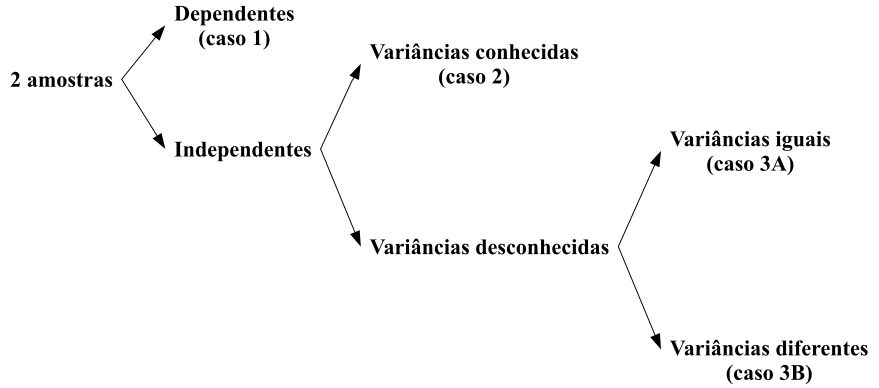
\includegraphics[width=1\linewidth]{figs/figure_9_1} \end{center}
\end{frame}

\setbeamercovered{transparent}
\begin{frame}
\frametitle{Resumo}

\textbf{Tabela 9.1: Comparação de médias para duas populações}

\begin{table}[h]
\tiny
\begin{tabular}{|c|c|}
\hline
Situação  & Estimadores  \\
\hline
Amostras Pareadas (Caso 1)  & 
\parbox{1cm}{\begin{align*}
\bar{D} &= \frac{\sum_i^nD_i}{n} \\
S^2_D &= \frac{1}{n-1}\sum_{i=1}^n(D_i-\bar{D})^2 \\
T &= \frac{\bar{D}-\mu_D}{S_D/\sqrt{n}} \sim t_{(n-1)}
\end{align*}}  \\
\hline
Amostras Independentes (Caso 2) Variâncias conhecidas  & 
\parbox{1cm}{\begin{align*}
\bar{D} &= \bar{X}-\bar{Y} \\
Var(\bar{D}) &= \sigma^2_X/n_1 + \sigma^2_Y/n_2 \\
Z &= \frac{\bar{D}-\mu_D}{\sqrt{\sigma^2_X/n_1 + \sigma^2_Y/n_2}}
\end{align*}} \\
\hline
\end{tabular}
\end{table}
\end{frame}

\setbeamercovered{transparent}
\begin{frame}
\frametitle{Resumo}
\textbf{Tabela 9.1: Comparação de médias para duas populações}
\begin{table}[h]
\tiny
\begin{tabular}{|c|c|}
\hline
Situação  & Estimadores  \\
\hline
Amostras Independentes (Caso 3A) Variâncias desconhecidas e iguais  &  \parbox{1cm}{\begin{align*}
\bar{D} &= \bar{X}-\bar{Y} \\
S^2_c &= \frac{(n_1-1)S^2_X+(n_2-1)S^2_Y}{(n_1-1)+(n_2-1)} \\
T &= \frac{\bar{D}-\mu_D}{\sqrt{S^2_c(1/n_1 + 1/n_2)}}
\end{align*}} \\
\hline
Amostras Independentes (Caso 3B) Variâncias desconhecidas e diferentes  & \parbox{1cm}{\begin{align*}
\bar{D} &= \bar{X}-\bar{Y} \\
\hat{\sigma}_{\bar{D}}^2 &= S^2_X/n_1+S^2_Y/n_2 \\
T &= \frac{\bar{D}-\mu_D}{\sqrt{S^2_X/n_1+S^2_Y/n_2}}
\end{align*}}  \\
\hline

\end{tabular}
\end{table}
\end{frame}

\setbeamercovered{transparent}
\begin{frame}
\frametitle{Exemplo 9.7}
Digitadores são treinados em uma empresa em duas turmas distintas. Na primeira, denominada Turma J, utiliza-se um método japonês de ensino, ao passo que na segunda turma, denominada Turma A, utiliza-se um método alemão. Dezesseis (16) alunos de cada turma foram escolhidos aleatoriamente e uma mesma tarefa foi atribuída a cada uma. Apesar de desconhecida as variâncias populacionais são consideradas iguais com base em estudos anteriores. Os métodos diferem quanto ao tempo de execução da tarefa? 

\begin{table}[h]
\tiny
\centering
\begin{tabular}{ccccccccccccccc}
\hline
Turma &  &  &  &  &  &  & Tempo &  &  &  &  &  &  &   \\
\hline
J & 10 & 13 & 9 & 10 & 14 & 13 & 10 & 15 & 12 & 10 & 9 & 10 & 13 & 14 \\
\hline
A & 15 & 12 & 18 & 16 & 15 & 17 & 17 & 15 & 16 & 17 & 11 & 17 & 14 & \\
\hline
\end{tabular}
\end{table}
 
\end{frame}

\setbeamercovered{transparent}
\begin{frame}
\frametitle{Referências bibliográficas}
\printbibliography
\end{frame}

\end{document}